\chapter{背景}\label{chap:background}

本章では、本論文の背景であるユーザのコンテキストを元に提供されるサービス・アプリケーション、および提案について述べる

\newpage


\section{Context-basedなサービス・アプリケーションの発展}

近年、スマートフォンと呼ばれるモバイルデバイスは、一般的な携帯物となっている。
スマートフォンが共通して持つセンサの種類は豊富になってきており、それらのセンサから取得したデータを利用した
ユーザの位置情報、行動履歴、ユーザの持つモバイルデバイス同士間の近接情報など、
ユーザの持っているコンテキストに基づく(Context-basedな)サービスを提供するアプリケーションもまた一般化してきている。

Foursquare\cite{foursquare}, Swarm\cite{swarm}は、GPSセンサからユーザの位置情報を読み取り、
現在居る位置情報に関連付けられた施設などの情報とユーザを結びつけて共有するサービスを提供している。
Firechat\cite{firechat}, Highlight\cite{highlight}は、
デバイス間の近接情報に基づき、使用するユーザー間とのコミュニケーション機能を提供している。
また、ゲームデバイスの分野でも、Nintendo DS\cite{3ds}やPS Vita\cite{vita}は、
すれ違い通信と呼ばれるユーザ同士が近接している状態から、無線通信によるユーザー同士のコミュニケーション機能を提供している。

以上のようなデバイスのセンサによりユーザのコンテキストを取得し、利用するアプリケーションは、今後も発展していくと思われる。

\begin{figure}[h]
    \begin{center}
        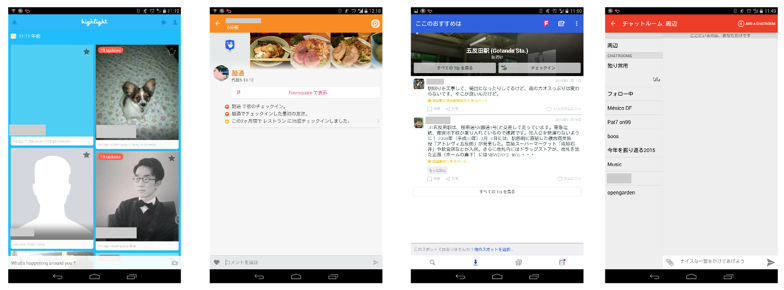
\includegraphics[width=1.0\linewidth]{img/contexts.eps}
    \end{center}
    \caption{Context-basedなサービス・アプリケーション}
    \label{fig:contexts}
\end{figure}


\section{今居るその場への情報共有手法}

人がその場に居合わせた他の人々へ情報を共有する、逆にその場に居合わせた人々から情報を取得する手法は、様々なものを検討することができる。

一般的なメールやSNSに依存したメッセージツールを使うのは、相手の連絡先をあらかじめ知っておく必要がある。
情報を共有したいが、個人間でなくその場を共有する多数の人間との共有を望んでいる場合、
個人の連絡先をまず共有するという手法は、プライバシーの面で安全とは言いがたい。
そのやりとりにはまず、個人間に十分な信頼が必要となる。
また、誰か一人が全体への共有を行うために連絡手法を呼びかけることもあるが、
誰もが偶然居合わせただけの状況では、集団を管理するのは難しいだろう。
その呼びかけも、誰もが自由に共有を行うプラットフォームとしては、手間の面で不便である。

その場を共有するための会場として設定する場合、NFCやWifiなどの機器を設置することによって共有のための空間を構築する手法は、
場に機器を設置する必要があり、何の設定もされていない場や、突発的な人間の集まりの場には対応することが難しくなる。

GPSセンサを使用した手法は、人々が携帯するモバイルデバイスには大抵の場合機能として含まれている上、
衛生から発信される電波を受信して測位を行うGPSには、場所を選ばないこともあり、一般的なセンサとして認識されている。
GPSの即位は広い距離範囲や平面的な距離測位において有効な効果を有するが、
測位の環境や電波状況などによって測位精度に影響が及ぶことにより、GPSは近距離での確実性を持った近接センサとは言い難い。

また、wifiによるアドホックな通信を行う手法では、昨今のモバイルデバイスの仕様上、
wifiのポートを通信中一つ専有することになるため、他の操作を阻害する恐れがある。
wifiのポートを2つ持つことが前提となるデバイスは、汎用的な手段としては選択し難い。

先行研究\cite{山本伶:2013-03-06}では、時限式で構造が変化するURLを共有することで
その場に居合わせた人間に対して情報を共有し、後からも変更、閲覧が可能な手法が提案されている。
本論文では、更に共有するためのキーワードも無く情報共有を行うことを可能にし、
あらかじめ名前の付いた場として設定されておらず、突発的な集団行動や普段の生活圏内の中でも情報共有が可能なサービスアプリケーションの提案を行う。


\section{近接情報取得手段としてのBluetooth無線技術}

Bluetooth\cite{bluetooth}は、GPSセンサと同じくモバイルデバイスに標準的に搭載されているモジュールである。
Bluetoothは電池持ちもいいし安価だし近接検出にとっても適してるよね

fireChat\cite{firechat}では、近接したデバイスとデバイスが、
インターネット回線に依存せずに通信しあうチャットコミュニケーション機能を有している。

Bluetoothを利用した、
ユーザが持つモバイルデバイス同士が近接したことを知るための
様々なアプリケーション\cite{すれちがったー}\cite{encountme}\cite{Monac}が存在する。



\section{デバイスによるアドホック通信}

\subsection{Bluetooth MANET}

MANETとは、Mobile Ad Hoc Networkの略称である。
MANET上のデバイスは上下左右、自由に移動可能な携帯性のあるデバイスである。
メッシュ・ネットワークの一つで、
通信拠点を介さず、デバイス同士でネットワークを構築して通信を行う。

アドホックネットワークとは、無線で接続可能な端末同士が専用の基地局やアクセスポイントを必要とせずに
通信を行う端末間のみで形成する無線ネットワークのことである。
通信にサーバを介さないため、インターネットに接続できない場所・状況でも相手ピアさえいれば通信が可能である。

そしてここで挙げるBluetooth MANETとは、Bluetoothによって築かれるMANETである。
Bluetoothの検出機能とペアリングを行って構築されるMANETであり、
一般的なAndroidモバイルデバイスに含まれるBluetoothは10mが検出範囲である。
この検出範囲は数珠つなぎのようにデバイスを連携させていくことによって検出範囲を広げていくことが可能で、この技術はホッピングと言われる。
先行研究ではBluetooth MANETによるものが提案されているが、
Bluetooth MANETはデバイスのペアリングが必要であり、ペアリングにはデバイス同士の認証が必要である。

また、Bluetooth4.0のプロトコルからは認証の必要が無い通信が可能となっている。
しかし、この通信でやりとり可能なデータ量はBluetoothによってペアリングしたデバイスや、インターネットに繋がっているデバイスに比べたら貧弱であり、
この手法が強力なのはインターネットが制限されている場合に限る。

本研究ではインターネットへの接続が制限されている状況を想定していないため、アドホックネットワークを用いず、
Bluetoothは近接するデバイスを検出する用途のみに利用する。
